% AST2000 Part 6: preparing for the landing (low orbit, spectrum, atmosphere, landing site).
% Compile: cd "Project 6/paper" && latexmk -pdf part6.tex   (or: python build_papers.py 6 from the repo root)
% Every number written as \val{key} comes from results.tex, made by pro_6.py.
\documentclass[aps,prd,twocolumn,nofootinbib,floatfix,superscriptaddress]{revtex4-2}
\usepackage{../../common/paper/ast2000}
\usepackage{tikz}
\usetikzlibrary{arrows.meta,positioning,shapes.geometric}
\tikzset{
  box/.style={draw, rounded corners=2pt, align=center, font=\footnotesize, inner sep=3pt, text width=#1},
  box/.default=6.6cm,
  decision/.style={draw, diamond, aspect=2.6, align=center, font=\footnotesize, inner sep=1pt},
  flow/.style={-{Stealth[length=2mm]}, thick}}

\begin{document}

\title{Part 6: Preparing for the Landing on Planet \val{dest}}
\author{Sakarias Frette}
\affiliation{AST2000 Rerun, University of Oslo}
\date{\today}

\begin{abstract}
Before landing, we study planet \val{dest} from orbit.
\begin{itemize}
\item \textbf{Low orbit.} A Hohmann descent brings the spacecraft from \val{start-radius}\,km to a circular orbit \val{low-alt}\,km above the surface. We choose that altitude by measuring the air drag directly: we flew test orbits at \val{probe-n} altitudes and recorded how fast each one decays. The decay falls off with a scale height of \val{probe-H}\,km.
\item \textbf{Composition.} A $\chi^2$ search of a 10-million-point spectrum, calibrated against pure noise, detects CH$_4$, CO and H$_2$O. All their lines share a Doppler shift of \val{v-common}\,km/s. O$_2$ is marginal in the spectrum.
\item \textbf{Atmosphere model.} The model is adiabatic up to \val{h-iso}\,km and isothermal above. We test it against air densities measured from the orbital decay. These require a mean molecular weight of $\mu=\val{mu-probe}\pm\val{mu-probe-err}$, which agrees with the composition that includes O$_2$ ($\mu=\val{mu-adopted}$) and rules out the one without it ($\mu=\val{mu-detected}$, \val{probe-ratio-detected}$\times$ too dense). The same drag data favour uniform gravity in the model.
\item \textbf{Spin.} Drag on a retrograde test orbit measures the planet's spin, giving a rotation period of \val{P-rot-drag}\,h (catalogue: \val{P-rot-api}\,h).
\item \textbf{Landing site.} We derive the coordinates of a point on the spinning surface at any time and scout one orbit of pictures. We choose an equatorial site where the star stands \val{site-sun}$^\circ$ high at the next pass overhead.
\end{itemize}
\end{abstract}

\maketitle

% =====================================================================
\section{Introduction}
Landing needs three things we do not yet have.
\begin{itemize}
\item A starting orbit close to the planet (\cref{sec:low}).
\item A model of the atmosphere, which will brake the lander. It needs the composition, from a spectrum (\cref{sec:spectrum}), and a physical model of how density falls with height (\cref{sec:atmos}).
\item A landing site, with its coordinates on a spinning planet (\cref{sec:sites}).
\end{itemize}
Throughout, we command the spacecraft through \code{ast2000tools}' \code{LandingSequence}~\cite{ast2000tools}.
It works in SI units relative to the planet's centre and does not track fuel, so we keep our own fuel account with the rocket equation.
We start from the Part 5 orbit with \val{fuel-start}\,kg of fuel.
Solar system seed: \val{seed}.

% =====================================================================
\section{Entering a low orbit}\label{sec:low}
\subsection{Method}
For the descent from $r_1$ to $r_2$ we set the velocity at $r_1$ to the apoapsis speed of the transfer ellipse,
\begin{equation}
  v_{\rm apo}=\sqrt{GM\left(\frac{2}{r_1}-\frac{1}{a}\right)},\qquad a=\frac{r_1+r_2}{2},
\end{equation}
fall for $\pi\sqrt{a^3/GM}$, and circularise with $v=\sqrt{GM/r_2}$.

How low is safe?
Drag removes orbital energy.
For a circular orbit in air that co-rotates with the planet (Part 7), the drag force $F=\tfrac12\rho C_dAv_{\rm rel}^2$ with $C_d=1$ shrinks the orbit by
\begin{equation}
  \Delta a_{\rm orbit}=2\pi\rho\,\frac{A}{m}\,a^2\left(\frac{v_{\rm rel}}{v}\right)^2 \label{eq:decay}
\end{equation}
per orbit.
We therefore probe the atmosphere with the spacecraft itself.
We enter circular test orbits at \val{probe-n} altitudes between 150 and 2000\,km and watch each for \val{probe-orbits} orbits.
These are test runs of the landing simulator; the flight restarts afterwards.

\subsection{Results}
\Cref{fig:probe} shows the measurement.
\begin{itemize}
\item At \val{probe-lowest-ok}\,km and below, drag wins and the API ends the run.
\item From \val{probe-fit-lo} to \val{probe-fit-hi}\,km the decay falls exponentially, with a scale height of $H=\val{probe-H}$\,km.
\item Higher up, only the integrator's numerical drift of \val{probe-floor}\,m per orbit remains.
\end{itemize}
The decay drops to \val{decay-limit}\,m per orbit at \val{edge}\,km.
We put the low orbit \val{safety-heights} scale heights higher, at \val{low-alt}\,km, where drag is twenty times weaker.

The descent costs \val{dv-descent} and \val{dv-circ}\,m/s, or \val{fuel-descent}\,kg of fuel, leaving \val{fuel-low}\,kg (\cref{fig:descent}).
Over \val{check-orbits} orbits in the new orbit, the semi-major axis changes by only \val{low-a-change}\,m, which is the integrator's drift, and $e<\val{low-e-max}$ (\cref{fig:low}).

\widefig{a1_descent}{The Hohmann descent from the Part 5 orbit to the low orbit, in the planet frame and as altitude against time.}{fig:descent}
\widefig{a2_drag_probe}{Drag probe. Radius lost per orbit against altitude, the exponential fit, and the chosen low orbit.}{fig:probe}
\widefig{a3_low_orbit}{The low orbit over \val{check-orbits} orbits, from the spacecraft's own orientations.}{fig:low}

% =====================================================================
\section{Spectral analysis of the atmosphere}\label{sec:spectrum}
\subsection{Theory}
The spacecraft moves at most $v_{\max}=\val{v-max}$\,km/s relative to the atmosphere, so a line at $\lambda_0$ can be shifted by at most
\begin{equation}
  \Delta\lambda_{\max}=\lambda_0\frac{v_{\max}}{c},
\end{equation}
which is \val{dl-632}\,nm at 632\,nm and \val{dl-2870}\,nm at 2870\,nm.
Each molecule's velocity along the line of sight is Gaussian with $\sigma_v=\sqrt{kT/m}$ (Part 1).
Since $\Delta\lambda/\lambda_0=v/c$, the line profile is a Gaussian of width
\begin{equation}
  \sigma=\frac{\lambda_0}{c}\sqrt{\frac{kT}{m}}. \label{eq:width}
\end{equation}
For O$_2$ at 632\,nm and 150--450\,K, that is \val{w-o2-150}--\val{w-o2-450}\,nm: only 2--3 data points, given the grid step of \val{step}\,nm.

\subsection{Method}
Each line is modelled as
\begin{equation}
  F=1+(F_{\min}-1)\,e^{-(\lambda-\lambda_c)^2/2\sigma^2}
\end{equation}
and fitted by minimising
\begin{equation}
  \chi^2=\sum_i\left(\frac{f_i-F(\lambda_i)}{\sigma_i}\right)^2.
\end{equation}
The noise $\sigma_i$ varies between \val{noise-min} and \val{noise-max} along the spectrum (\cref{fig:spectrum}).
Four ideas make the analysis fast and objective.

\paragraph{Exact depth.}
The model is linear in the depth $A=F_{\min}-1$.
For each $(\lambda_c,\sigma)$ the best depth is $A^*=S_{fg}/S_{gg}$, with $S_{fg}=\sum w(f-1)g$, $S_{gg}=\sum wg^2$ and $w=1/\sigma_i^2$.
As functions of $\lambda_c$ both sums are convolutions with a Gaussian kernel.
The whole $(\lambda_c,T)$ grid therefore costs one convolution per temperature.
A least-squares fit then refines the minimum and gives uncertainties.

\paragraph{Calibrated threshold.}
A $\chi^2$ fit always finds \emph{some} line.
To know what noise alone can do, we run the identical search on \val{n-noise-windows} line-free stretches of the spectrum near each line.
A line counts as detected only if its $\Delta\chi^2=\chi^2_{\rm no\,line}-\chi^2_{\rm best}$ beats noise with a false-alarm probability below \val{false-alarm}.

\paragraph{Two stages.}
A blind search over all $\pm\val{v-max}$\,km/s gives the strong lines and their common Doppler shift.
A second search looks only within $\pm\val{v-width}$\,km/s of that shift.
With far fewer places for noise to hide, its threshold is much lower: it corrects for the look-elsewhere effect.

\paragraph{Completeness.}
We inject synthetic lines of known depth into the noise to see how deep a line must be for us to find it.

The procedure is summarised in \cref{fig:flowB}.

\begin{figure}[tbp]\centering
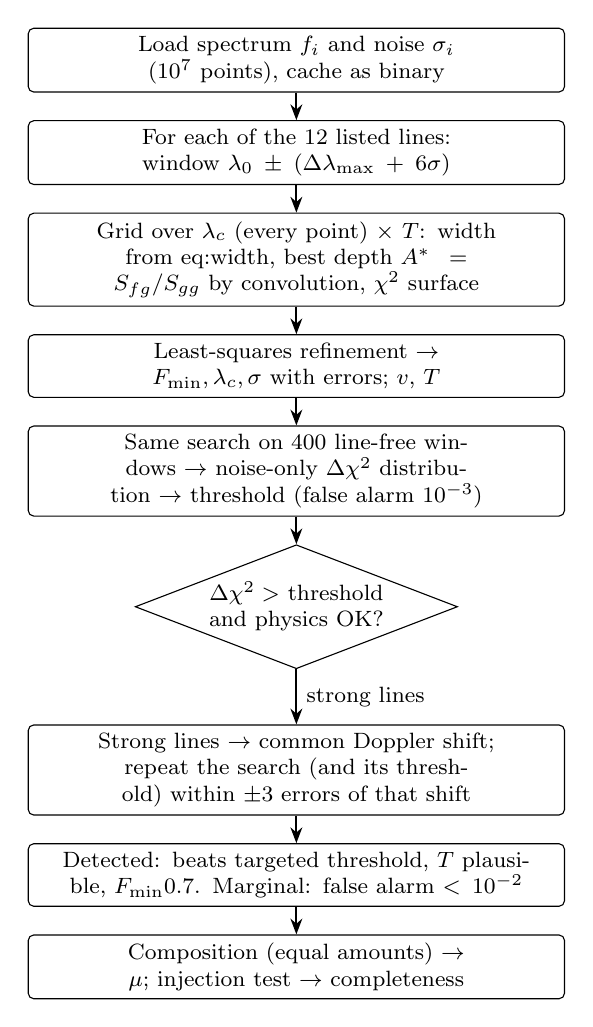
\begin{tikzpicture}[node distance=3.5mm]
\node[box] (load) {Load spectrum $f_i$ and noise $\sigma_i$ (10$^7$ points), cache as binary};
\node[box, below=of load] (win) {For each of the 12 listed lines: window $\lambda_0\pm(\Delta\lambda_{\max}+6\sigma)$};
\node[box, below=of win] (grid) {Grid over $\lambda_c$ (every point) $\times$ $T$: width from \cref{eq:width}, best depth $A^*=S_{fg}/S_{gg}$ by convolution, $\chi^2$ surface};
\node[box, below=of grid] (fit) {Least-squares refinement $\to F_{\min},\lambda_c,\sigma$ with errors; $v$, $T$};
\node[box, below=of fit] (noise) {Same search on 400 line-free windows $\to$ noise-only $\Delta\chi^2$ distribution $\to$ threshold (false alarm $10^{-3}$)};
\node[decision, below=of noise] (blind) {$\Delta\chi^2>$ threshold\\and physics OK?};
\node[box, below=7mm of blind] (shift) {Strong lines $\to$ common Doppler shift; repeat the search (and its threshold) within $\pm$3 errors of that shift};
\node[box, below=of shift] (verdict) {Detected: beats targeted threshold, $T$ plausible, $F_{\min}\gtrsim0.7$. Marginal: false alarm $<10^{-2}$};
\node[box, below=of verdict] (mu) {Composition (equal amounts) $\to\mu$; injection test $\to$ completeness};
\draw[flow] (load) -- (win); \draw[flow] (win) -- (grid); \draw[flow] (grid) -- (fit);
\draw[flow] (fit) -- (noise); \draw[flow] (noise) -- (blind);
\draw[flow] (blind) -- node[right, font=\footnotesize] {strong lines} (shift);
\draw[flow] (shift) -- (verdict); \draw[flow] (verdict) -- (mu);
\end{tikzpicture}
\caption{Flowchart of the spectral analysis (challenge B).}\label{fig:flowB}
\end{figure}

\subsection{Results}
The blind search finds \val{n-blind} lines far above their thresholds, with $\Delta\chi^2$ against threshold:
\begin{itemize}
\item CH$_4$ 1660\,nm: \val{CH4-1660-blind} vs.\ \val{CH4-1660-blind-thr};
\item CH$_4$ 2200\,nm;
\item CO 2340\,nm: \val{CO-2340-blind} vs.\ \val{CO-2340-blind-thr};
\item H$_2$O 940\,nm: \val{H2O-940-blind} vs.\ \val{H2O-940-blind-thr}.
\end{itemize}
All four share a Doppler shift of $\val{v-blind}\pm\val{v-blind-err}$\,km/s (\cref{fig:fits,fig:evidence}).
That agreement alone is strong evidence that they are real: flukes land anywhere in $\pm\val{v-max}$\,km/s.
The detected gases are \val{gases}, which gives $\mu=\val{mu-detected}$.

\paragraph{The O$_2$ question.}
At 760\,nm the fitted line sits at the common shift (\val{O2-760-v}\,km/s), with $\Delta\chi^2=\val{O2-760-dchi2}$.
That is just below the targeted threshold of \val{O2-760-thr}, so it counts as marginal.
Its $F_{\min}=\val{O2-760-Fmin}\pm\val{O2-760-Fmin-err}$ is below the expected 0.7.
It lies where the noise is \val{O2-760-noise-at} times its median, and noise there can deepen a real line as easily as it can fake one.

The completeness test explains why O$_2$ is hard to see.
All three O$_2$ lines lie in noisy parts of the spectrum.
There, our search finds a line with 90\% reliability only if it is deeper than about 0.3 (\cref{fig:completeness}), deeper than real lines are expected to be.
The spectrum therefore cannot exclude O$_2$, whereas CO$_2$ and N$_2$O lines deeper than about 0.13 would have been found.
\Cref{sec:atmos} settles the O$_2$ question with an independent measurement.

The temperatures from the line widths are poorly constrained (lines only 2--3 points wide).
They agree with 150--450\,K only within their large errors.

\widefig{b1_spectrum}{The whole spectrum (binned) with the listed lines and verdicts, and the noise $\sigma_i$ along it.}{fig:spectrum}
\widefig{b2_line_fits}{Every listed line in its window on a Doppler-velocity axis, with the targeted fit. Green: detected.}{fig:fits}
\widefig{b3_chi2_maps}{$\chi^2$ against Doppler velocity and temperature for the strongest lines (contours: 1, 2, 3$\sigma$).}{fig:chi2}
\widefig{b4_evidence}{Real lines or flukes. Significance in the blind and targeted searches against noise-only thresholds; blind Doppler velocities; temperatures.}{fig:evidence}
\colfig{b5_completeness}{Fraction of injected lines recovered against their depth, for every line position.}{fig:completeness}

% =====================================================================
\section{A model of the atmosphere}\label{sec:atmos}
\subsection{Theory}
We combine
\begin{itemize}
\item hydrostatic equilibrium, $\dd P/\dd h=-\rho g$;
\item the ideal gas law, $P=\rho kT/\mu m_u$;
\item the adiabatic relation $P^{1-\gamma}T^\gamma=$ const, with $\gamma=\val{gamma}$, below the height where $T=T_0/2$, and constant $T$ above.
\end{itemize}
Together these give
\begin{align}
  \frac{\dd T}{\dd h}&=-\frac{\gamma-1}{\gamma}\frac{\mu m_ug}{k}\ \text{(adiabatic)},\quad 0\ \text{(isothermal)},\\
  \frac{\dd\ln\rho}{\dd h}&=-\frac{\mu m_ug}{kT}-\frac{1}{T}\frac{\dd T}{\dd h}.
\end{align}
The boundary conditions are $T_0=\val{T0}$\,K (Part 3) and $\rho_0=\val{rho0}$\,kg/m$^3$ (\code{ast2000tools}).
With uniform gravity the solution has a closed form: $T$ falls linearly, $\rho=\rho_0(T/T_0)^{1/(\gamma-1)}$, and then $\rho$ falls exponentially with $H=k(T_0/2)/(\mu m_ug_0)$.

\subsection{Method}
We integrate $(\ln\rho,T)$ upward with an adaptive Runge--Kutta solver.
The solver stops exactly where $T=T_0/2$ (an event) and continues isothermally.
\code{density(h)} and \code{temperature(h)} interpolate the solution (\cref{fig:flowC}).
Run with uniform gravity, it matches the closed form to \val{closed-form-check}.

We then compare the model with the drag probe.
Inverting \cref{eq:decay} with the spacecraft's mass and area turns each measured decay into a density (\val{n-probe-heights} heights, \val{probe-h-lo}--\val{probe-h-hi}\,km).
We fit $\mu$ to those densities.

\begin{figure}[tbp]\centering
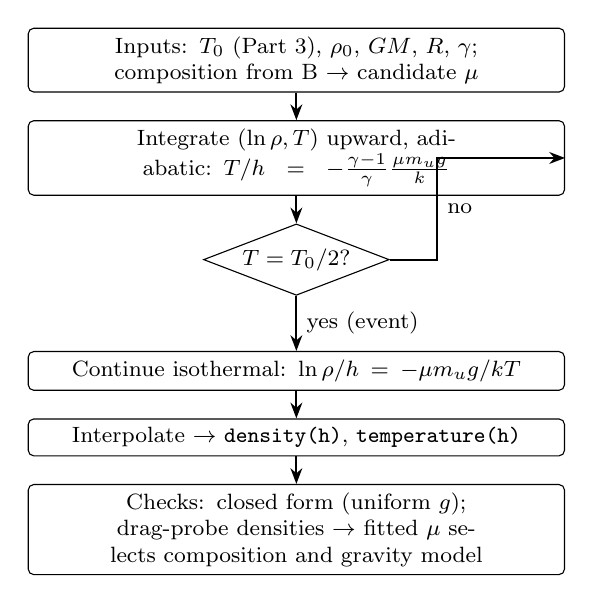
\begin{tikzpicture}[node distance=3.5mm]
\node[box] (in) {Inputs: $T_0$ (Part 3), $\rho_0$, $GM$, $R$, $\gamma$; composition from B $\to$ candidate $\mu$};
\node[box, below=of in] (ad) {Integrate $(\ln\rho,T)$ upward, adiabatic: $\dd T/\dd h=-\frac{\gamma-1}{\gamma}\frac{\mu m_u g}{k}$};
\node[decision, below=of ad] (ev) {$T=T_0/2$?};
\node[box, below=7mm of ev] (iso) {Continue isothermal: $\dd\ln\rho/\dd h=-\mu m_ug/kT$};
\node[box, below=of iso] (spl) {Interpolate $\to$ \texttt{density(h)}, \texttt{temperature(h)}};
\node[box, below=of spl] (chk) {Checks: closed form (uniform $g$); drag-probe densities $\to$ fitted $\mu$ selects composition and gravity model};
\draw[flow] (in) -- (ad); \draw[flow] (ad) -- (ev);
\draw[flow] (ev) -- node[right, font=\footnotesize] {yes (event)} (iso);
\draw[flow] (ev.east) -- ++(0.6,0) |- node[pos=0.25, right, font=\footnotesize] {no} (ad.east);
\draw[flow] (iso) -- (spl); \draw[flow] (spl) -- (chk);
\end{tikzpicture}
\caption{Flowchart of the numerical atmosphere model (challenge C).}\label{fig:flowC}
\end{figure}

\subsection{Results}
\Cref{fig:drag} is the key result.
\begin{itemize}
\item With uniform gravity, the drag densities require $\mu=\val{mu-probe}\pm\val{mu-probe-err}$.
\item Only the composition that includes the marginal O$_2$ agrees ($\mu=\val{mu-adopted}$): the model then matches the measured densities to a median factor of \val{probe-ratio-adopted} over four decades.
\item Without O$_2$ ($\mu=\val{mu-detected}$) the model is \val{probe-ratio-detected} times too dense.
\end{itemize}
We therefore adopt \val{composition}.
The two independent measurements agree: a marginal spectral line, and the air density weighed by the spacecraft's orbit.

The same data also decide the gravity question.
Letting $g$ fall with height gives a scale height near 300\,km of \val{H-varying-300}\,km, against the measured \val{probe-H}.
It needs $\mu=\val{mu-probe-g}$, matching no allowed composition, and it fits twice as badly.
Gravity is \val{g-drop-100}\% weaker at 100\,km, a small change.
Its effect on density compounds over many scale heights, however (\cref{fig:gravity}): a factor of \val{uniform-ratio-100} at 100\,km and \val{uniform-ratio-300} at 300\,km.
We adopt uniform gravity, as the assignment allows and the data prefer.

The adopted atmosphere (\cref{fig:profiles}):
\begin{itemize}
\item at the surface: \val{P0}\,bar and \val{rho0}\,kg/m$^3$;
\item adiabatic up to \val{h-iso}\,km, cooling at \val{lapse}\,K/km;
\item isothermal above, at \val{T-iso}\,K, with $H=\val{H-iso}$\,km;
\item density \val{rho-100}\,kg/m$^3$ at 100\,km and \val{rho-low}\,kg/m$^3$ at our low orbit.
\end{itemize}

\subsection{After the fact: the API's own atmosphere}
Everything above was decided from measurements alone.
Afterwards we read the atmosphere that \code{ast2000tools} uses internally (\cref{fig:api}).
These are private attributes, so we kept them out of every decision.
\begin{itemize}
\item \textbf{Molecule mass:} \val{api-mu-mp} proton masses, or \val{api-mu-u}\,u. Our adopted value is \val{api-mu-err}\% off, and the drag measurement alone is \val{api-probe-err}\% off.
\item \textbf{Composition:} 23.5 is exactly $(32+18+16+28)/4$, i.e.\ O$_2$, H$_2$O, CH$_4$ and CO in equal amounts. O$_2$ is really there.
\item \textbf{Other parameters:} the API uses $T_0=\val{api-T0}$\,K (the same black-body formula as Part 3), $C_d=\val{api-Cd}$ and uniform gravity.
\end{itemize}
Our density profile matches the API's to \val{api-rho-ratio-100} at 100\,km and \val{api-rho-ratio-300} at 300\,km, and the temperature to within \val{api-T-diff}\,K.
Had we trusted only the spectrum's clear detections, the density at 300\,km would have been \val{api-detected-ratio-300} times too high.

\widefig{c1_profiles}{Temperature, density and pressure against height. Numerical model, closed form, and the variant with gravity falling with height.}{fig:profiles}
\widefig{c2_drag_check}{Left: densities measured by orbital decay against the model for each allowed composition. Right: $\mu$ of each composition against the $\mu$ fitted to the drag data.}{fig:drag}
\widefig{c3_gravity}{How good is uniform gravity? $g(h)$, and the ratio of densities with real and uniform gravity.}{fig:gravity}
\widefig{c4_api_check}{After the fact: our density and temperature against the API's hidden atmosphere, and the parameters side by side.}{fig:api}

% =====================================================================
\section{Scouting for landing sites}\label{sec:sites}
\subsection{Coordinates on a spinning planet}
We use spherical coordinates $(r,\theta,\phi)$ as in Part 4, in the planet-centred landing frame.
The planet spins about $z$ with $\omega=2\pi/P_{\rm rot}$, so a point fixed on the surface keeps $r$ and $\theta$ and
\begin{equation}
  \phi(t_0+\Delta t)=\phi(t_0)+\omega\,\Delta t .
\end{equation}
The function \code{new_coordinates} implements this for any number of points and times at once.

Two checks make sure this is right.
\begin{itemize}
\item \textbf{The frame.} Part 5's last state in the solar-system frame equals the landing sequence's first one to \val{frame-miss}\,m, so the axes are shared.
\item \textbf{The spin.} At \val{spin-alt}\,km a retrograde test orbit, which meets the co-rotating air faster, decays \val{decay-ratio} times faster than a prograde one (\cref{fig:spin}). Solving $(v+\omega a)^2/(v-\omega a)^2$ for $\omega$ gives $P_{\rm rot}=\val{P-rot-drag}$\,h, against \val{P-rot-api}\,h from \code{ast2000tools}. That is \val{spin-err}\% off, and it confirms counterclockwise spin.
\end{itemize}

\subsection{Scouting}
During one low orbit, with the camera pointing straight down, we take \val{n-pictures} pictures (MCAst files \code{site_k.xml}).
For each we record the point below, its planet-fixed longitude, and the star's elevation there, from the planet's position on its orbit (Kepler, Part 2).
The spacecraft passes over a given site every
\begin{equation}
  \left(\frac{1}{P_{\rm orbit}}-\frac{1}{P_{\rm rot}}\right)^{-1}=\val{pass-period}\,\mathrm{h}
\end{equation}
(\cref{fig:rotation}).
The lander will come down near such a pass.
For every site we therefore compute the next pass after scouting, and the star's elevation then.

\subsection{Result}
\val{n-lit} of the \val{n-pictures} sites are in daylight at their next pass.
We choose site \val{site-index} on the equator ($\theta=\val{site-theta}^\circ$, planet-fixed $\phi=\val{site-phi}^\circ$ at $t=0$).
It is passed overhead at $t=\val{site-pass}$\,h, when the star stands \val{site-sun}$^\circ$ high (\cref{fig:scouting}), close to local noon.
At that time it sits at $\phi=\val{site-phi-pass}^\circ$ in the landing frame.
The coordinates are saved for Part 7.
The pictures can be inspected in MCAst to veto bad terrain; the code takes a manual choice instead if needed.

\widefig{d1_frame_and_spin}{Frame check and drag measurement of the planet's spin.}{fig:spin}
\widefig{d2_scouting}{Left: the planet seen from above its north pole in the planet-fixed frame, with day and night at the landing pass and the pictured sites. Right: star elevation at each site over one planet day, with the next pass overhead.}{fig:scouting}
\widefig{d3_rotation}{The coordinate function at work: longitudes of the site and the spacecraft in the landing frame, and their separation with the predicted passes.}{fig:rotation}

% =====================================================================
\section{Discussion and conclusion}
The most valuable tool in this part was one we built ourselves: using the spacecraft's own orbital decay as an instrument.
It gave four results.
\begin{itemize}
\item A safe orbit altitude.
\item The atmosphere's scale height.
\item The planet's spin.
\item The absolute air density, decisive for the composition. The spectrum alone could not settle O$_2$: its lines fall where the noise is worst. A density measurement that needs $\mu\approx\val{mu-probe}$ could.
\end{itemize}

The main uncertainties are as follows.
\begin{itemize}
\item \textbf{Assumed abundances.} Equal amounts of each gas are assumed, as instructed; the true abundances could differ.
\item \textbf{Line temperatures.} These are poorly constrained.
\item \textbf{The model's structure.} $T_0$ comes from a black-body estimate, and the atmosphere is assumed to be adiabatic, then isothermal. The drag check tests all of these together in the upper atmosphere, not separately, and not near the surface where the landing happens.
\end{itemize}
Comparing with the API's hidden atmosphere afterwards confirms the model to within 2\% below 300\,km.
The landing site (site \val{site-index}) is confirmed for Part 7.

\bibliography{../../common/paper/references}

\appendix
\section{Mission log}
\begin{missionbox}{Part 6 key numbers (seed \val{seed})}
Low orbit & \val{low-alt}\,km, period \val{low-period}\,min \\
Fuel left & \val{fuel-low}\,kg \\
Drag scale height & \val{probe-H}\,km \\
Detected / marginal gases & \val{gases} / \val{marginal-gases} \\
Common Doppler shift & \val{v-common}\,km/s \\
Adopted composition, $\mu$ & \val{composition}, \val{mu-adopted} \\
$\mu$ from drag & \val{mu-probe}$\pm$\val{mu-probe-err} \\
Surface $P$, $\rho$, $T$ & \val{P0}\,bar, \val{rho0}\,kg/m$^3$, \val{T0}\,K \\
Rotation period (drag) & \val{P-rot-drag}\,h \\
Landing site & equator, $\phi=\val{site-phi}^\circ$ (planet-fixed) \\
\end{missionbox}

\end{document}
